\section{FreeRTOS}
\begin{itemize}
    \item Developed and maintaned by Real Time Engineers Ltd.
    \item Supports 23 microcontroller architectures
    \item Small footprint (4.3Kbytes on an ARM7)
    \item Written in C
    \item Preemptive tasks
    \item Unlimited number of tasks and priorities
    \item Implements queues, binary/counting semaphores and mutexes
\end{itemize}

\subsection{Tasks}

\subsubsection{Task States}
\begin{minipage}{0.6\textwidth}
    \begin{description}
        \item[Running] When a task is actually executing it is said to be in the Running state.
              It is currently utilising the processor.
        \item[Ready] Ready tasks are those that are able to execute (they are not in the Blocked or Supsended state) but are not currently executing because a different tas of equal or higher priority is already in the Running State.
        \item[Blocked] A task is said to be in the Blocked state if it is currently waiting for either a temporal or external event.
              For example, if a task call \texttt{vTaskDelay()} it will block until the delay period is expired - a temporal event.
              Tasks can also block to wait for a queue, semaphore, event groupt, notification or semaphore event.
        \item[Suspended] Like tasks that are in the Blocked state, tasks in the Suspended state cannot be selected to enter the Running state, but tasks in the Suspended state do not have a time out.
              Instead, tasks only enter or exit the Suspended state when explicitly commanded to do so through the \texttt{vTaskSuspend()} and \texttt{xTaskResume()} API calls respectively.
    \end{description}
\end{minipage}
\begin{minipage}{0.4\textwidth}
    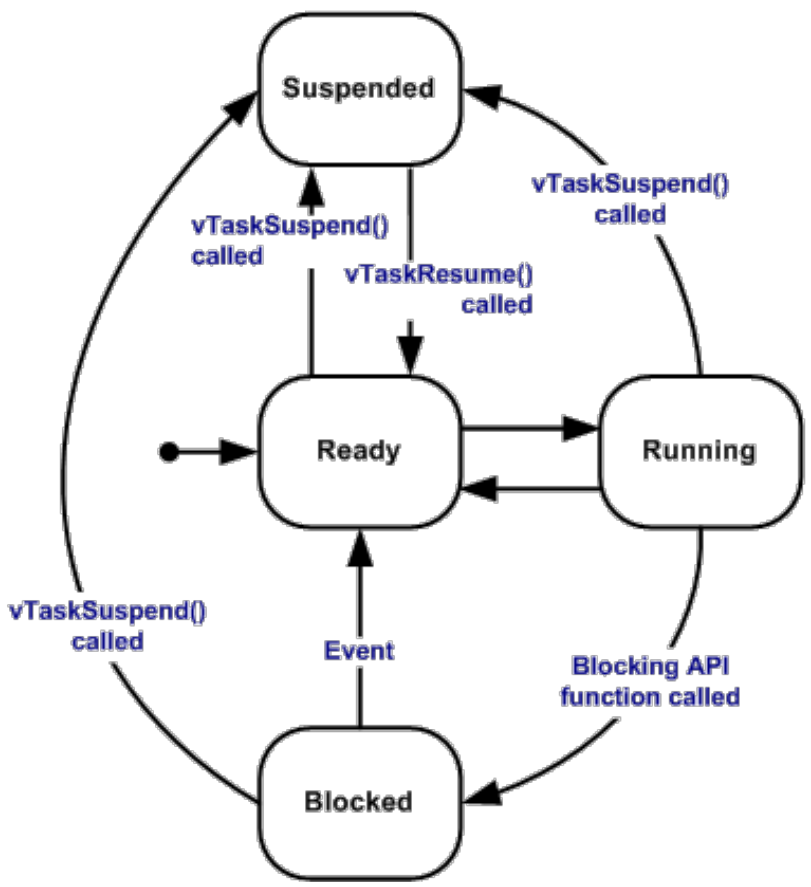
\includegraphics[width=1\textwidth]{images/RTOS/task_states_freertos.png}
\end{minipage}


\subsubsection{Task creation}
% \columnratio{0.5}
% \begin{paracol}{2}
\lstinputlisting[style=C, lastline=8]{snippets/FreeRTOS/task_creation.c}
% \switchcolumn
\lstinputlisting[style=C, firstline=10]{snippets/FreeRTOS/task_creation.c}
% \end{paracol}

\subsection{Communication}
\subsubsection{Pipes}
In FreeRTOS pipes are called Stream Buffers or Message Buffers

\subsubsection{Queues}
\lstinputlisting[style=C]{snippets/FreeRTOS/queue_functions.c}


\subsection{Resource Sharing}

\subsubsection{Semaphores}
\lstinputlisting[style=C]{snippets/FreeRTOS/semaphore_functions.c}

\subsubsection{Mutexes}
\lstinputlisting[style=C]{snippets/FreeRTOS/mutex_functions.c}

\subsubsection{Issue Solving in FreeRTOS}
Only supports priority inheritance (enable it in FreeRTOSConfig.h).
Further recommendation: Implement a tas with queue, \textbf{FreeRTOS Gatekeeper Task}.